The system consists of three logically separate components as illustrated in
Figure~\ref{fig:system_overview}; 1) the equipment component where all
communication with apparatus and acquisition of data is performed 2) the servers
which consists of the MySQL server that stores the acquired data from
experiments by the apparatus used and the webserver which interacts and
presents the user with data retrieved from the database and 3) the user
component which is made up of the clints whishing to access the data.
\begin{figure}
 \begin{center}
 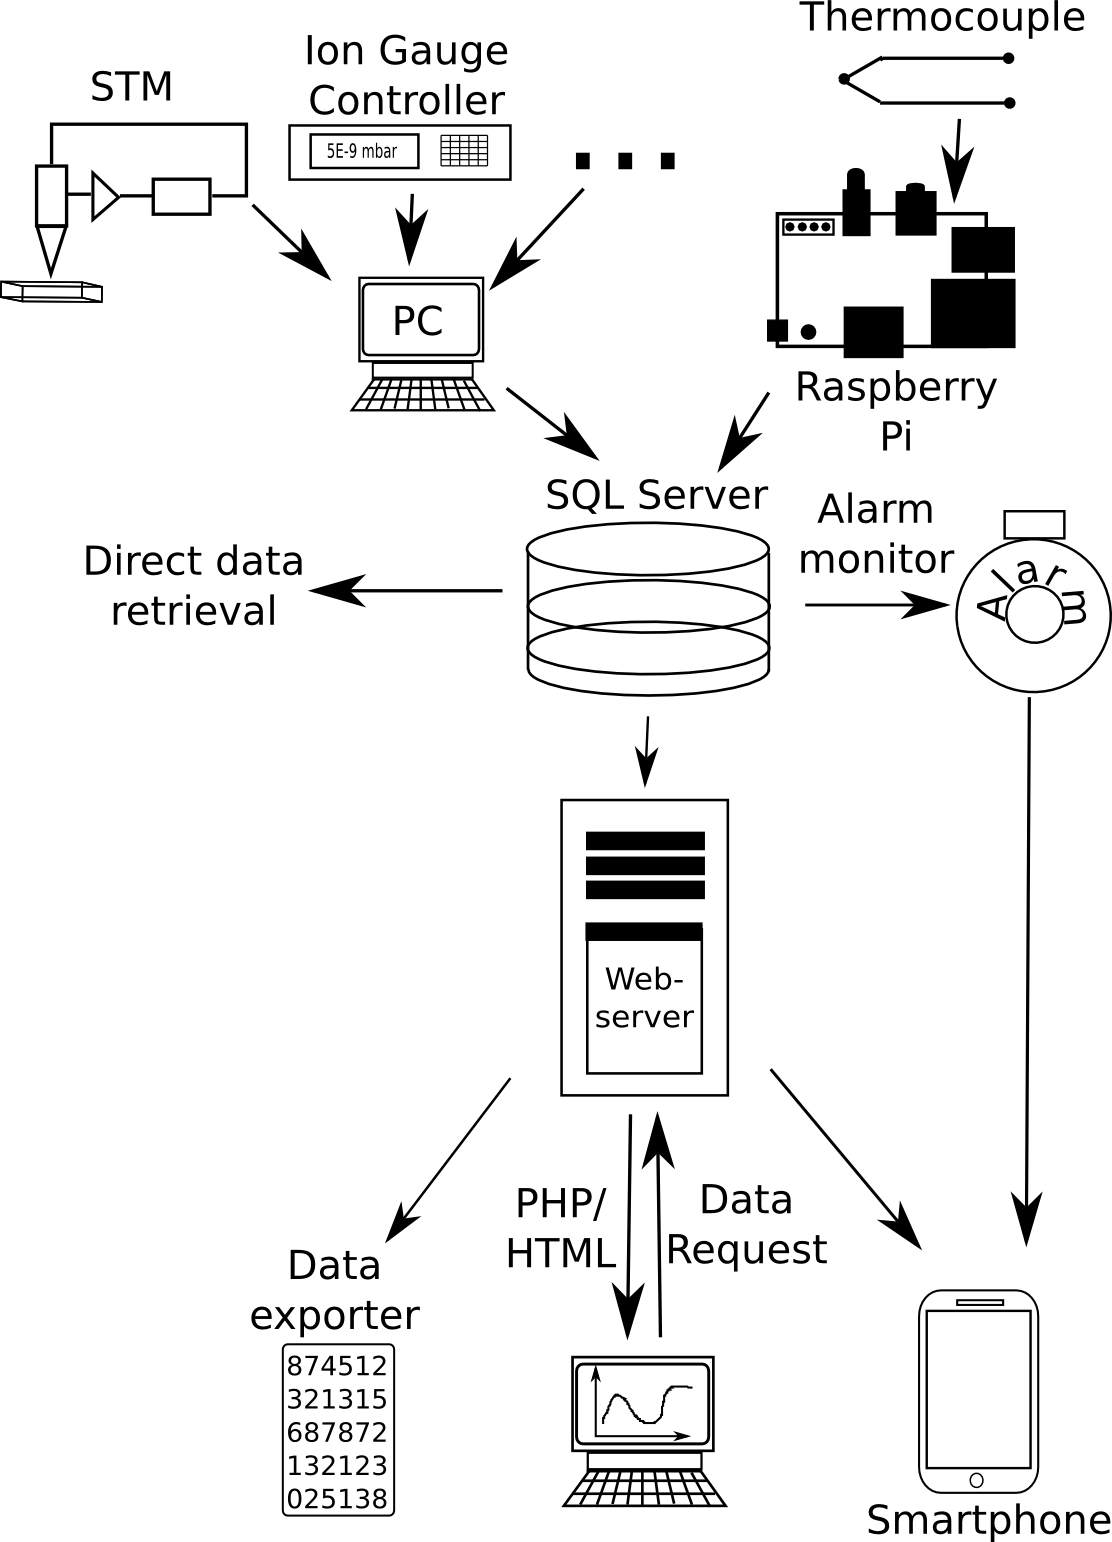
\includegraphics[width=10cm]{system_overview.png}
 \caption{
   A schematic representation of the structure of data handling system.
   \label{fig:system_overview}
 } 
 \end{center}
\end{figure}

The system is highly modular meaning the servers can accept data from a range
of different sources. In the current setup equipment interfaced with RS232,
GPIB, USB, analog/digital data acquisition cards standards written in both
Labview and Python runs on the server. How the integration with the server and
subsequent storage of data in the database is performed is hence a user
determined design decision. This has a number of attractive advantages. The
user(s) can integrate existing software with the databases quickly and without
the need to rewrite any previous interface software written for experimental
setups. Backup of experimental data on the local client is, from a user's point
of view, transparent as this can be performed by routine jobs on the server.

The servers consist of a MySQL server and a webserver. All experimental data is
stored on the MySQL server while most of the data is presented to the user from
the webserver. If needed, experimental data from the MySQL server can be
directly retrieved for later analysis. Furthermore, by logging experimental
data from clients continuously, alarm triggers can be used to warn users when
logged parameters fall out of range. The webserver runs a backed of Python/PHP
which is used to display the data to users via a website. Data is hence fetched
from the MySQL server by the webserver and subsequently presented for the user.
To accommodate a range of users and provide the largest flexibility the
webserver displays both a standard HTML/CSS site for desktop PCs and a mobile
version suitable for tablet/smartphone users.

Access for users is provided in two different ways. Either the user can use a
computer or a handheld device to access the data. The webinterface, with which
the user interacts, is also capable of routine data treatment. This can either
be range change of displayed data, plotting on a log scale, performing a
running average, etc. In this way the user can easily and quickly get an
overview of acquired data.
